\subsection{Описание работы FSK}

Frequency Shift Key - вид модуляции, при которой скачкообразно изменяется частота несущего сигнала в зависимости от значений символов информационной последовательности. Частотная модуляция весьма помехоустойчива, так как помехи искажают в основном амплитуду, а не частоту сигнала.

Для модулирования и тестирования данного процесса, необходимо построить следующую схему в графическом интерфейсе GNU Radio
    
    \begin{landscape}
	\begin{figure}[H]
		\centering
		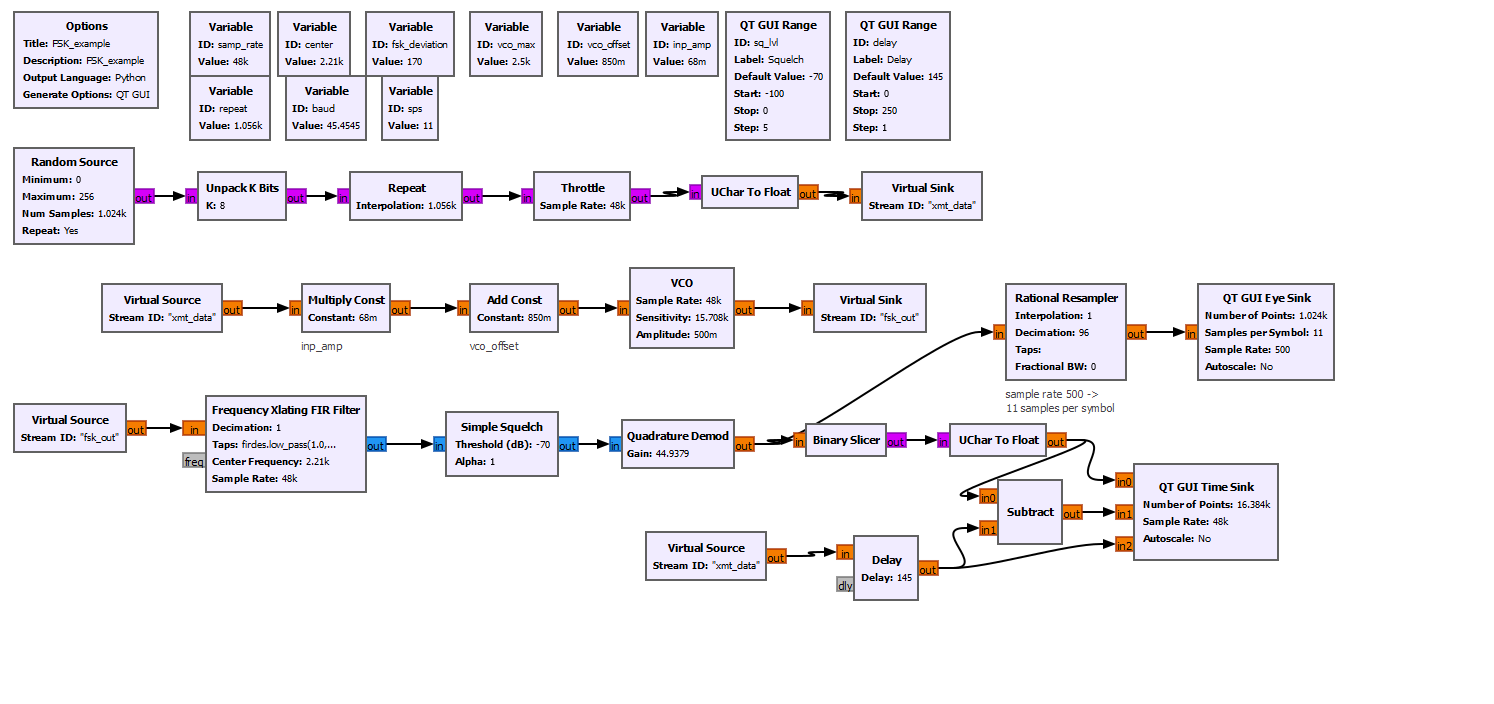
\includegraphics[width=25.5cm]{fig/lab12/lab12_1.png}
		\caption{Схема FSK}
		\label{pic:fsk_scheme} % название для ссылок внутри кода
	\end{figure}
\end{landscape}

В данной схеме используются следующие блоки:

\begin{itemize}
	\item Frequency Xlating FIR Filter - Этот блок выполняет частотный перевод сигнала, а также понижает разрешение сигнала, запуская на нем децимирующий FIR-фильтр.
	\item Simple Squelch - Простой блок шумоподавления на основе средней мощности сигнала и порога в дБ.
	\item Quadrature Demod - Этот блок вычисляет произведение одновыборочного отложенного и сопряженного входного сигнала и нераскрытого сигнала, а затем вычисляет аргумент (также известный как угол, в радианах) результирующего комплексного числа.
	\item Binary Slicer - Нарезает числа с плавающей запятой, производя 1-битный вывод. Положительный ввод производит двоичную 1, а отрицательный ввод производит двоичный ноль. 
	\item QT GUI Sink - Выводы необходимой инфомрации в графическом интерфейсе.
    \item Options - Этот блок устанавливает некоторые общие параметры графа потоков. Такие как название проекта, авторство и другие. 
	\item Variable - Этот блок сопоставляет значение с уникальной переменной. Есть возможность использования переменной в другом блоке, благодаря идентификатору (id) блока переменных. 
	\item Multiply Const - Умножает входной поток на скалярную или векторную константу.
	\item Add Const - Прибавляет к входному потоку скалярную или векторную константу.
	\item QT GUI Range - Этот блок создает переменную с выбором виджетов. Переменной может быть присвоено значение по умолчанию, и ее значение может быть изменено во время выполнения в указанном диапазоне.
	\item Random Source - Генератор случайных чисел.
	\item Unpack K bits - Преобразует байт с k релевантных битов в k выходных байтов с 1 битом каждый.
	\item Repeat - Количество раз для повторения входных данных, выступающих в качестве коэффициента интерполяции.
	\item Throttle - Этот блок служит для того, чтобы дросселировать поток так, чтобы средняя скорость не превышала удельную скорость.
	\item Uchar To Float - Преобразует unsigned chars в поток float.
	\item Virtual Sink - Служит для сохранения потока в вектор.
	\item Virtual Source - Работает в паре с Virtual Sink блоком. Источник данных, который передаёт элементы на основе входного вектора. 
	\item VCO - Генератор с регулируемым напряжением. Создает синусоиду частоты на основе амплитуды входного сигнала.
\end{itemize}

В этом примере используется Baudot Radioteletype, следовательно битовое время = 22 миллисекунды. Получаем скорость передачи 45,4545.
Коэффицент повторения равен samp\_rate * 0,022.

В VCO генерируются сигналы 2295 Гц (отметка = 1) и 2125 Гц (отметка = 0). При выборе полной шкалы частоты 2500 Гц (vco\_max) для входа +1 чувствительность VCO = (2 * math.pi * 2500 / 1) = 15708. Можно использовать любую частоту выше 2295 Гц. 2500 Гц — хорошее круглое число. Глядя на вывод виртуального источника «xmt\_data», Mark = +1.0 и Space = 0.0. Частота отметки 2295 Гц создается вектором inp\_amp = (1,0 * 0,068) + vco\_offset = 0,918, что равно (2295/2500). Параметр отводов частотного Xlating FIR Filter равен 'firdes.low\_pass(1.0,samp\_rate,1000,400)'.

Теперь посмотрим, что у нас с данными:
\quad Источник генерирует случайные байты (от 0 до 255). Далее этот байт распоковывается в каждый бит становится байтом со значащим младшим разрядом. Для ограничения потока использует Throttle.
\quad Приёмник при помощи фильтра смещает принимаемый сигнал так, чтобы он был сосредоточен вокруг центральной частоты - между частотами Mark и Space. Шумоподавитель добавлен для реального приёма сигналов. Блок Quadrature Demod производит сигнал, который является положительным для входных частот выше нуля и отрицательным для частот ниже нуля. Когда данные доходят до Binary Slicer, то на выходе получает биты, это и есть наша полученная информация.


\subsection{Тестирование}

    \begin{figure}[H]
	\begin{center}
		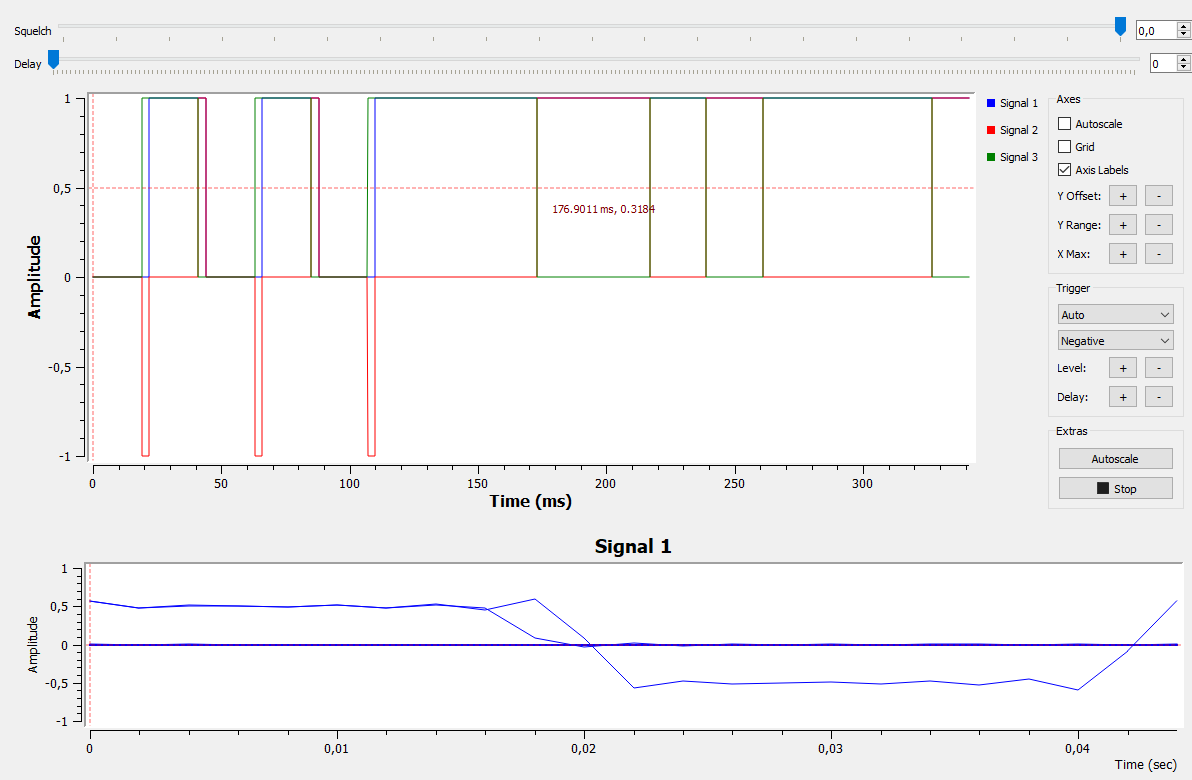
\includegraphics[scale=0.4]{fig/lab12/lab12_2.png}
		\caption{Модуляция без задержки и шума}
		\label{pic:e1} % название для ссылок внутри кода
	\end{center}
\end{figure}

На графике можно видеть 3 сигнала разного цвета. Зеленный показывает данные которые были переданы передатчиком. Синий - это данные полученные приемником. А красный отвечает за разницу между зеленым и синим. Красный сигнал должен быть равен нулю, это сигнализирует о том, что данные передаются верно, однако на диаграмме сверху видно, что это не так и выходит так, что полученная информация различается от той, которую передавали. Принятый сигнал находится на некоторое количество бит позади, потому что цепочка передатчика и приемника имеет много блоков и фильтров, которые задерживают сигнал. Для того чтобы это исправить необходимо сделать задержку между приемом и передачей данных, что и обеспечивает блок Delay. Правильном задержкой является 145. 

    \begin{figure}[H]
	\begin{center}
		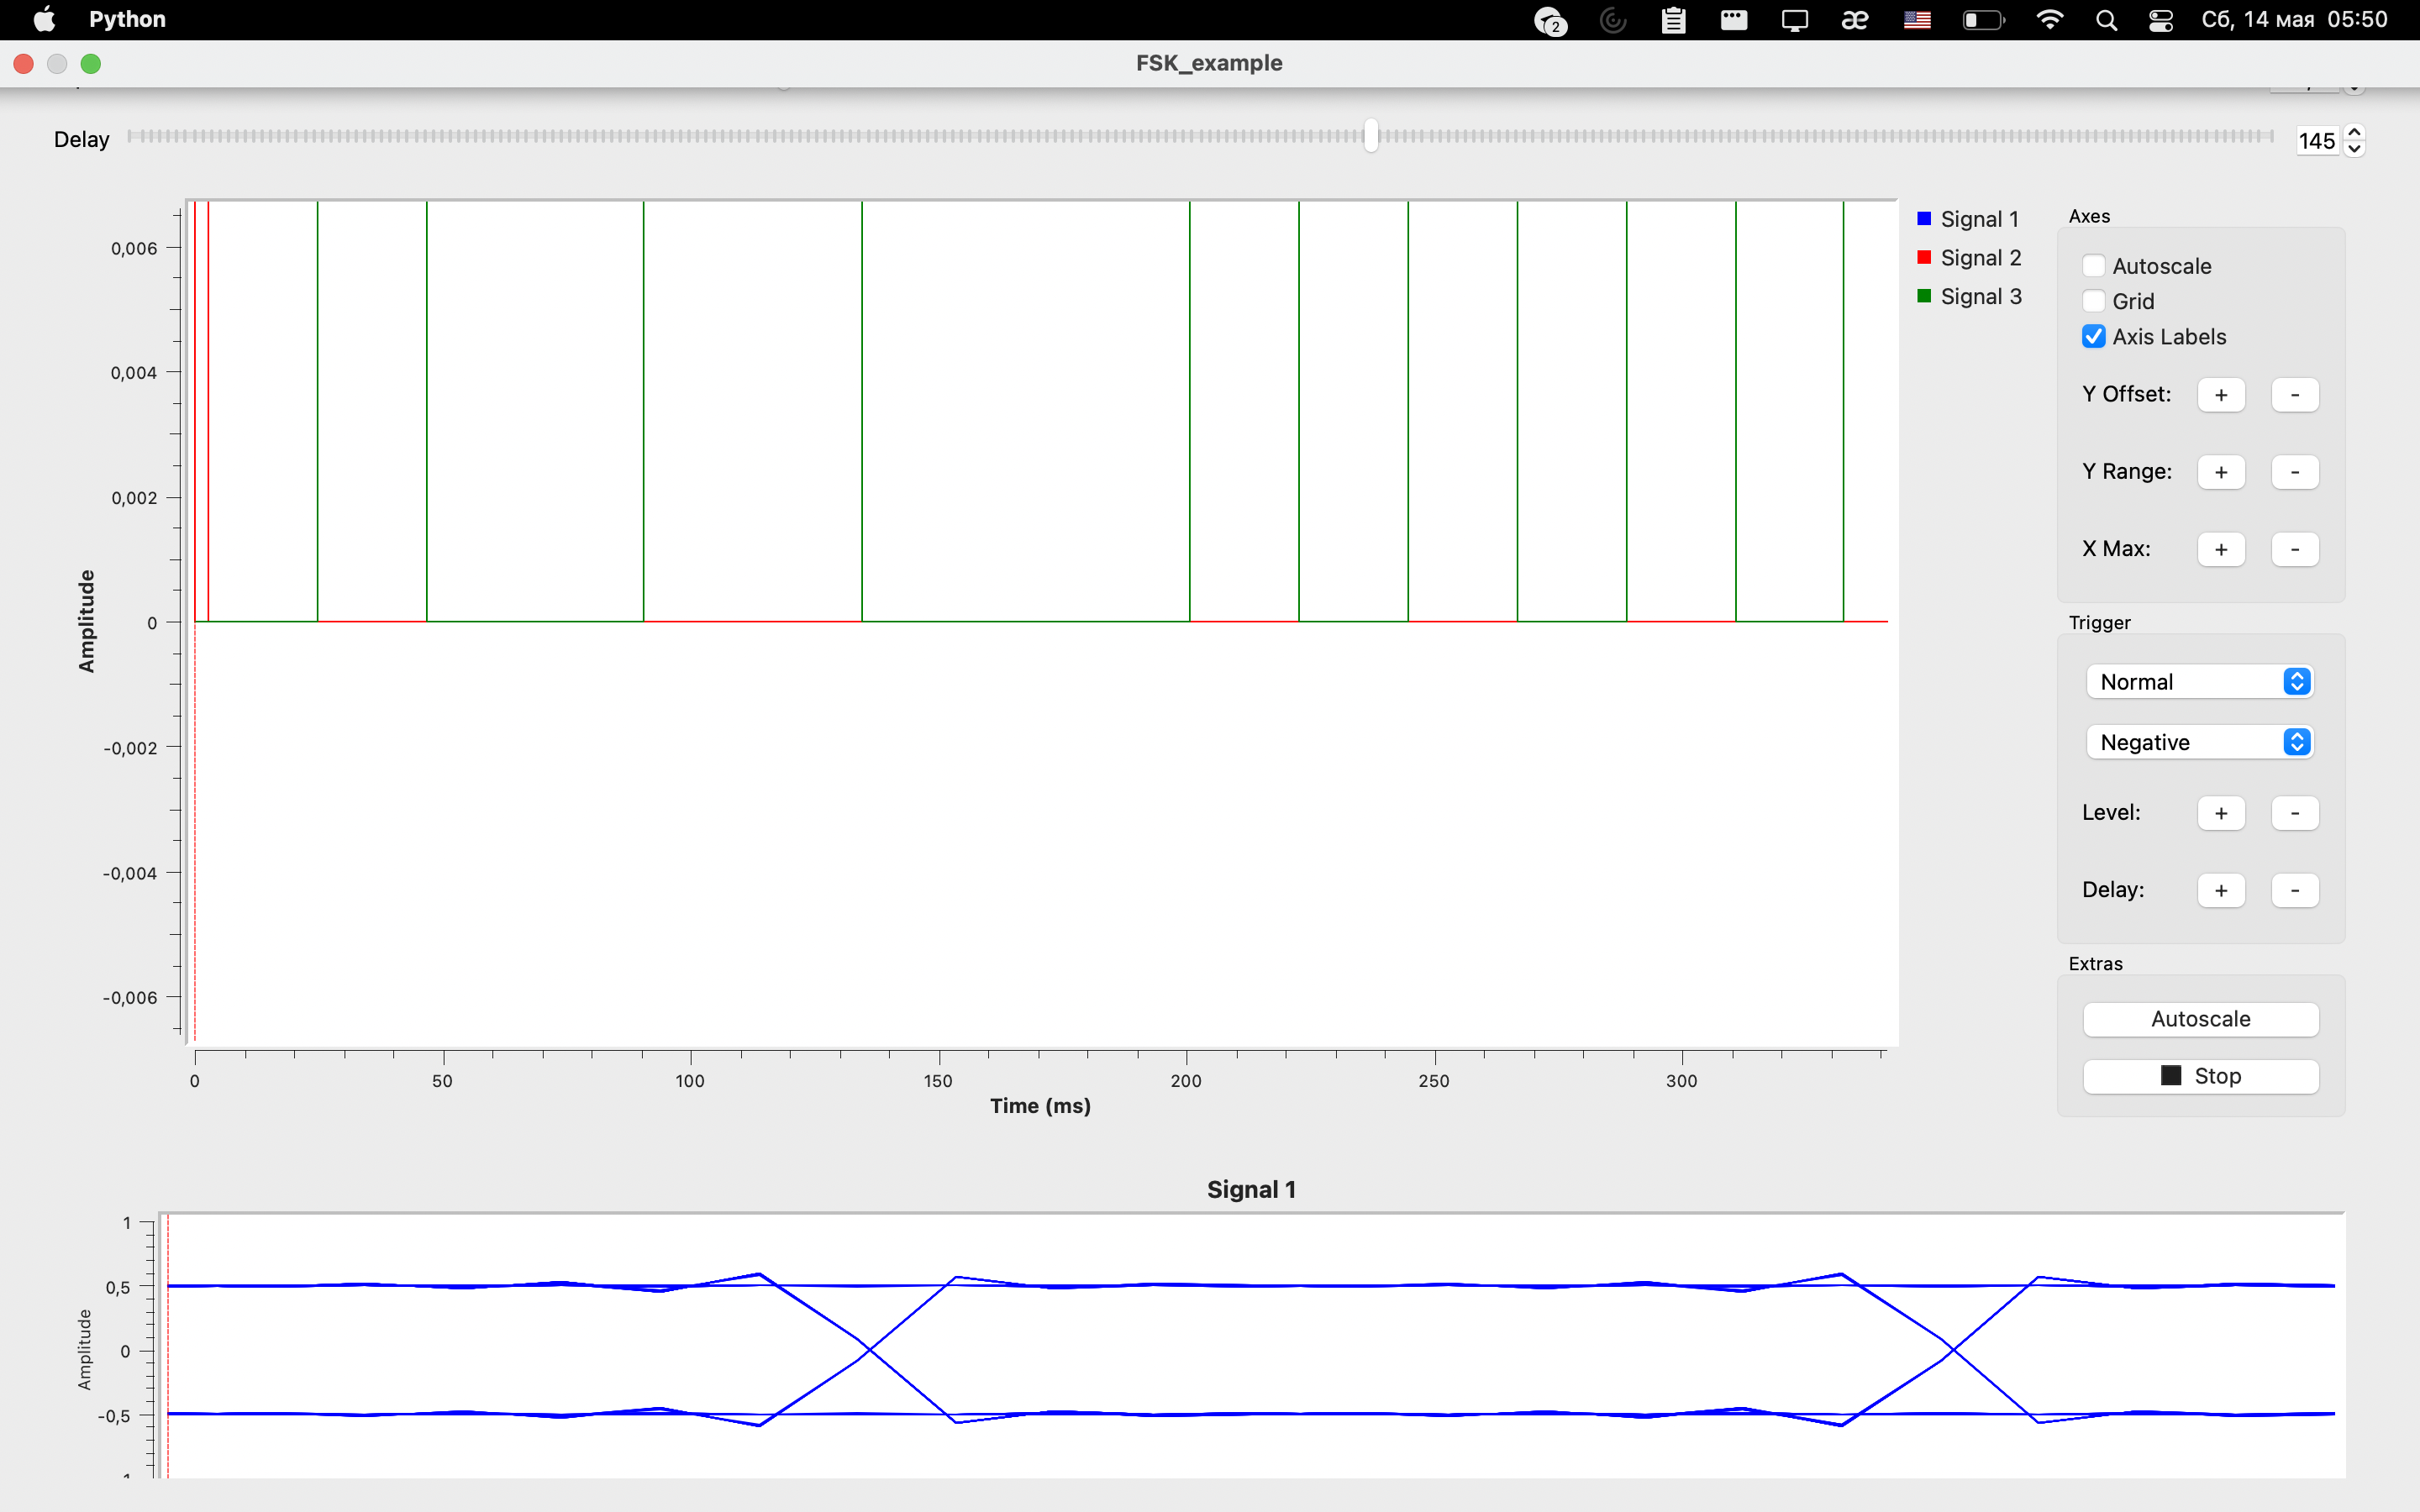
\includegraphics[scale=0.3]{fig/lab12/lab12_3.png}
		\caption{Модуляция с правильной задержкой}
		\label{pic:e2} % название для ссылок внутри кода
	\end{center}
\end{figure}

Теперь как можно заметить все хорошо и данные передаются и получаются корректно. 

\subsection{Вывод}
В данной лабораторной работе был рассмотрен один из способов модуляции. При помощи GNU Radio была создана и протестирована необходимая модель . 
